\section{Introduction}
Network on Chip (NoC) architectures enable high performance, scalable and power efficient multi-core systems for modern compute and communication intensive applications~\cite{Joshi2007,Neeb2005}.
Researchers have proposed different NoC topologies such as mesh, ring, torus, binary trees, star etc., each having varying degrees of quality of service, bandwidth and latency~\cite{Dally2003,Kumar2002}.
Despite their simple architecture and routing algorithms, binary trees are generally not attractive for NoC implementations.
It is mainly because of its lower bisection bandwidth.
Fat trees are proposed as a remedy to improve the bandwidth by adding more number of links when moving towards the root node.
This solution works well in traditional interconnect networks such as computer networks~\cite{Shainer2011}.
In an NoC environment, their advantage is limited since the switch complexity increses as the network size increases.
This limits the maximum supported clock frequency of the network thus bringing down the system performance. 

Theoretically instead of increasing the link width between tree levels, increasing the clock frequency between them should provide the same benefit.
In traditional computer networks this may not be possible since the network interfaces operate on predefined standards which restrict the frequency of operation.
In an NoC environment, this is very much possible since all the compute instances are within the same chip and are not restricted by any physical protocol. 
Modern FPGAs support asynchronous FIFOs, which make the implementation of such asynchronous switches easier.
These switches have simpler architecture than fat tree switches and support better clock frequency.
But they are more resource intensive compared to traditional binary trees.

\begin{figure}[t]
\centering
   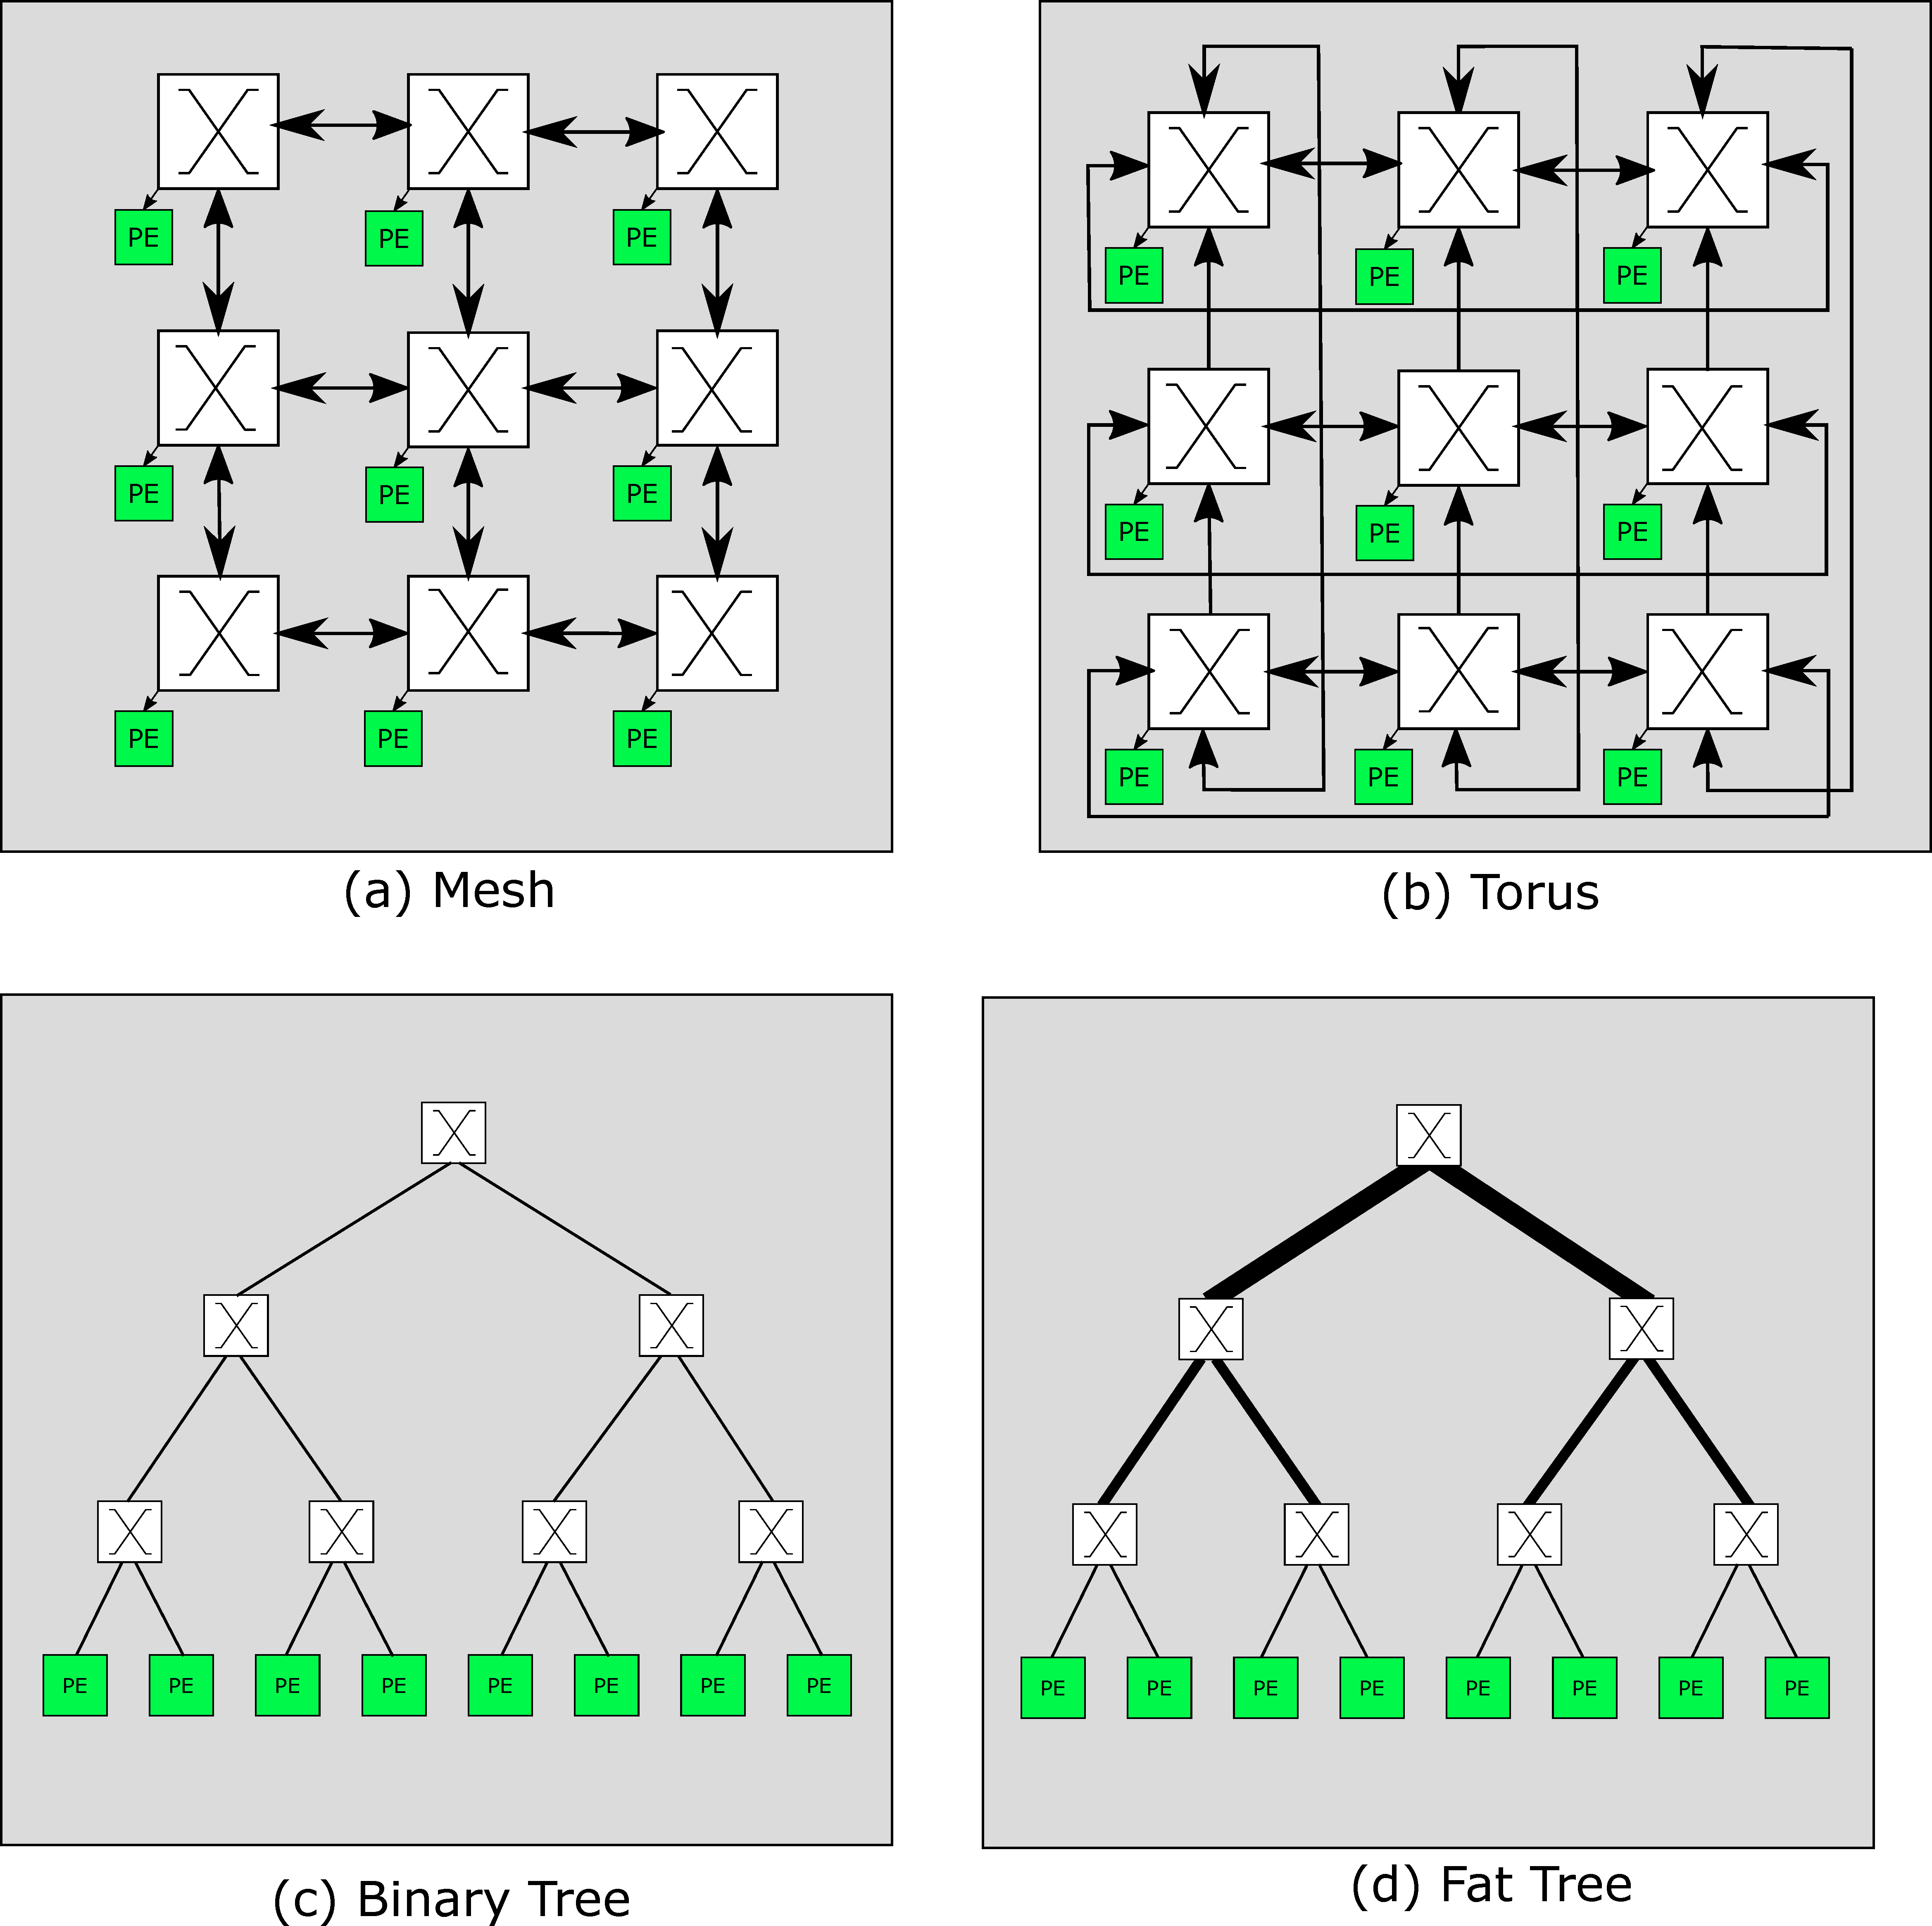
\includegraphics[width=\columnwidth]{Figures/topologies.pdf}
   \caption{Different NoC topologies}
   \label{fig:topologies}
\end{figure}


Although asynchronous NoCs are proposed before for integrated circuits, they are not evaluated for binary tree performance improvement~\cite{Bjerregaard2005, USP2011,Miro2007}. A quantitative analysis is missing in the literature especially for FPGA implementations.
In this work we present a quantitative analysis of different tree topologies namely the binary tree, binary fat tree and asynchronous binary tree when targeting FPGA based NoC implementation. 
The main contributions of this work are
\begin{itemize}
\item detailed design of an open-source globally asynchronous-locally synchronous (GALS) binary tree-based NoC implementation targeting Xilinx FPGAs,
\item performance evaluation of the proposed infrastructure with traditional binary trees and the state-of-the-art open source binary fat tree, torus and mesh topologies,
\item and an analysis of trade-off points for the different implementations when targeting FPGAs.
\end{itemize}
The remainder of this paper is organized as, Section~\ref{sec:background} discusses the relevant background, Section~\ref{sec:arch} discusses the architecture of the proposed NoC, Section~\ref{sec:result} discussed the performance metrics and ~\ref{sec:conclusion} concludes the paper and gives the future research directions.